% ----------------------------------------------------------------------------------------
%	PACKAGES AND THEMES
%----------------------------------------------------------------------------------------
\documentclass[xcolor=dvipsnames,t,9pt]{beamer}
%\documentclass[aspectratio=169,xcolor=dvipsnames,t,9pt]{beamer} %for 16:9 ratio slide
\usetheme{Symply}

\usepackage{hyperref}
\usepackage{graphicx} 
\usepackage{booktabs} 
\usepackage{multirow}
\urlstyle{same}
\usepackage{appendixnumberbeamer}

\setbeamertemplate{bibliography item}{[\arabic{enumiv}]}

%----------------------------------------------------------------------------------------
%	TITLE PAGE FOR RESEARCH PRESENTATION
%----------------------------------------------------------------------------------------

\title{Fairness-Aware Optimal Market Participation of \\Aggregated Distributed Energy Resources}
\subtitle{Final Project Proposal}
\author[장서현 $|$]{\textbf{장서현 (jangseohyun@yonsei.ac.kr)}\inst{1}} % set short author for author name in footline 
\institute[연세대학교 산업공학과] 
{
  \inst{1}\textbf{SY}stems \textbf{M}odeling and \textbf{P}rogramming \textbf{L}ab \\Department of Industrial Engineering, \textbf{Y}onsei University - \textbf{SYMPLY} \\
  (\url{https://symply.yonsei.ac.kr/})
}  % set short institute for department and institute in footline 
\date[IIE7585 확률적계획법 $|$]
{
    IIE7585 확률적계획법 (2025.05.28)\\\bigskip
    \centerline{\includegraphics[width=0.4\textwidth]{logo_text.png}}
} % set shortdate for conference title in footline


%----------------------------------------------------------------------------------------
%   기존 폰트 설정 부분
%----------------------------------------------------------------------------------------
% \usepackage[T1]{fontenc}
% \usepackage[usefilenames,DefaultFeatures={Ligatures=Common}]{plex-otf} %
% \renewcommand*\familydefault{\sfdefault} %% Only if the base font of the document is to be sans serif

% \usepackage[unfonts]{kotex}
% \xetexkofontregime{latin}[puncts=prevfont, colons=prevfont, cjksymbols=hangul]
% \setmainhangulfont{NanumSquare}
% \setsanshangulfont{NanumSquare}
% \setmonohangulfont{NanumSquare}

%NanumGothic, NanumSquare, Noto Sans CJK KR

%----------------------------------------------------------------------------------------
%   다른 방식의 폰트 설정 부분
%----------------------------------------------------------------------------------------
\usepackage{kotex}
\usepackage{fontspec}
\setsansfont{IBMPlexSans}[
    Path=./IBMPlexSans/,
    Extension = .ttf,
    UprightFont=*-Light,
    BoldFont=*-Medium,
    ItalicFont=*-LightItalic,
    BoldItalicFont=*-MediumItalic,
    ]
% Light and Medium from IBMPlexSansKR for both English and Korean
% LightItalic and MediumIntalic from IBMPlexSans for only English

% \usepackage{kotex}
% \usepackage{fontspec}
% \setsansfont{NotoSansKR}[
%     Path=./NotoSansKR/,
%     Extension = .ttf,
%     UprightFont=*-Light,
%     BoldFont=*-Light,
%     % ItalicFont=*-Italic,
%     % BoldItalicFont=*-BoldItalic,
%     ]



%----------------------------------------------------------------------------------------
%	PRESENTATION SLIDES
%----------------------------------------------------------------------------------------

\begin{document}

{
\setbeamertemplate{headline}{} % no headline on title page
\setbeamertemplate{footline}{} % no footline on title page
\begin{frame}[noframenumbering] % no page count on title page
    % Print the title page as the first slide
    \titlepage
\end{frame}
}

% {
% \setbeamertemplate{headline}{} % no headline on title page
% \setbeamertemplate{footline}{} % no footline on title page
\begin{frame}{목차} % no page count on title page
    % Throughout your presentation, if you choose to use \section{} and \subsection{} commands, these will automatically be printed on this slide as an overview of your presentation
    \tableofcontents
\end{frame}
% }

%------------------------------------------------
\section[문제 배경]{문제 배경}
%------------------------------------------------

\begin{frame}{분산에너지원 (Distributed Energy Resources, DER)}
    \textbf{에너지를 사용하는 공간ㆍ지역 또는 인근지역에서 공급하거나 생산하는 에너지로, 일정 규모 이하의 소규모 에너지 \cite{Korea2023DER}}
    \begin{itemize}
        \item 태양광(PV) 및 풍력 터빈(WT) 발전 장치, 에너지 저장 시스템(ESS), 전기 자동차(EV) 충전기, 마이크로그리드 등을 포함
        \item 소규모 발전의 형태에 적합한 탄소중립적인 에너지를 중심으로 생산
    \end{itemize}

    \begin{block}{}
        $\Rightarrow$ 불안정한 대규모 중앙집중식 송전 및 발전에서 벗어나, 수요지 인근에서 환경친화적이고 독립적인 에너지의 생산과 소비 가능
    \end{block}

\end{frame}

%------------------------------------------------

\begin{frame}{전력시장 (Wholesale Electricity Market)}
    \small
    \setlength{\columnsep}{0pt}
    \begin{columns}
        \column{0.5\textwidth}
        \raggedright
        \textbf{하루전시장 Day-ahead Commitment Market} \vspace{0.2em}
        \begin{itemize}
            \item 하루 전에 예측된 수요와 공급 기반으로 다음날 시간별 가격이 결정됨
            \item 공시된 가격에 따라 일정량의 전력 공급/소비를 \textbf{하루 전에 계약} (commitment)
            \item 계약 불이행 시 페널티 발생
        \end{itemize}
        \column{0.45\textwidth}
        \raggedright
        \textbf{실시간시장 Real-time Balancing Market} \vspace{0.2em}
        \begin{itemize}
            \item 실시간 수요와 공급 차이를 조정하는 시장
            \item 5분에서 20분 간격으로 \textbf{실시간 가격 책정 및 수급 조정}
            \item Day-ahead 시장가보다 평균적으로 낮으며, 가격 변동성이 큼
        \end{itemize}
    \end{columns}

    \vspace{7pt}

    \begin{figure}[htb!]
        \centering
        \begin{minipage}[t]{0.48\linewidth} % 동일한 너비 지정
            \centering
            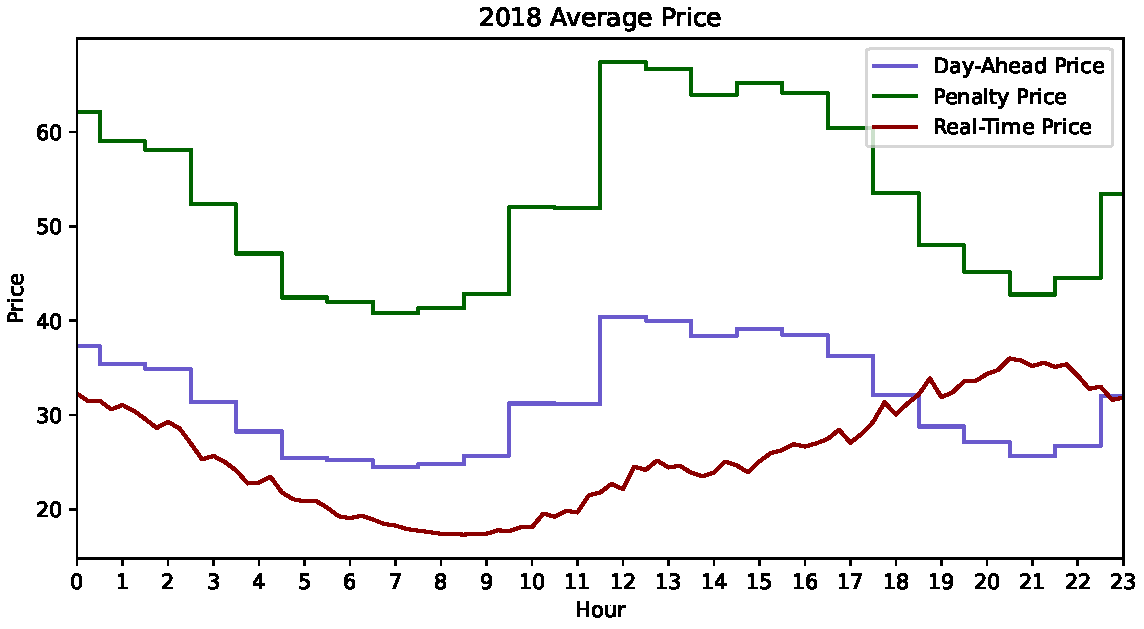
\includegraphics[width=\linewidth]{fig_avgprice.pdf}
            \caption{Annual Average Electricity Price \cite{pecanstreet}}
            \label{fig:avgprice}
        \end{minipage}
        \begin{minipage}[t]{0.48\linewidth} % 동일한 너비 지정
            \centering
            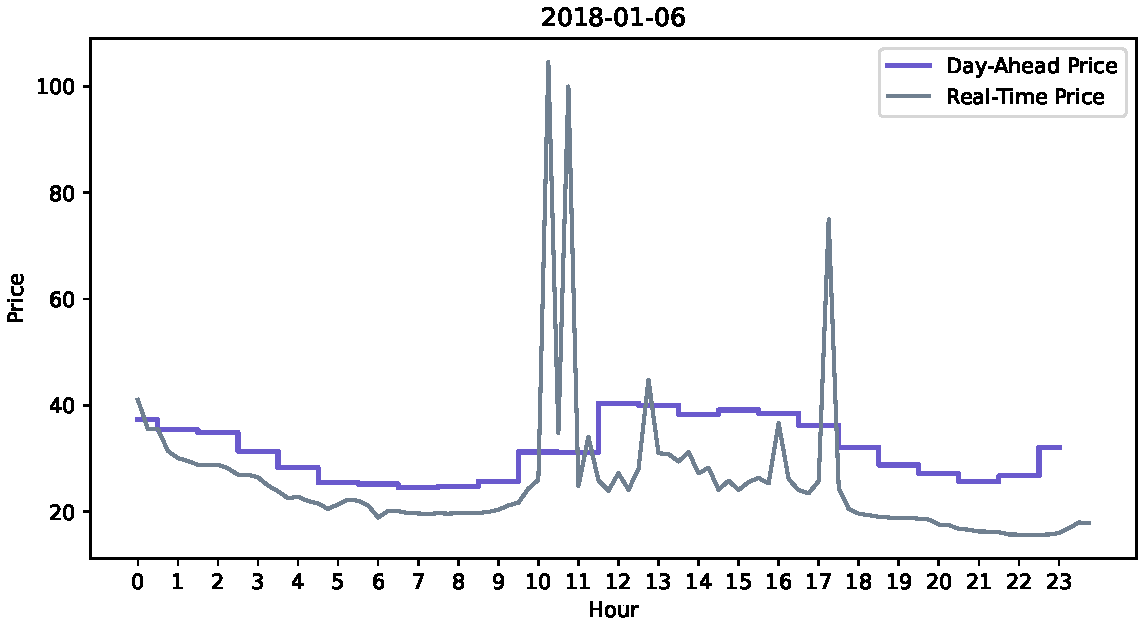
\includegraphics[width=\linewidth]{fig_price.pdf}
            \caption{Variability in Real-Time Price \cite{pecanstreet}}
            \label{fig:price}
        \end{minipage}
        \hfill % 두 이미지 사이 간격 조정
    \end{figure}

\end{frame}

%------------------------------------------------

\begin{frame}{분산에너지원의 통합 (Aggregation)}
    \textbf{여러 개별 분산에너지원들을 하나의 포토폴리오(Aggregated Distributed Energy Resources, ADER)로 통합하는 과정으로, 가상 발전소나 에너지 관리 시스템 등을 통해 구현}

    \begin{block}{Aggregation이 필요한 이유}
        \textcircled{\small{1}} 재생에너지 발전량의 불확실성과 \textcircled{\small{2}} non-dispatchable한 출력 특성으로 인해,\\ 안정적인 day-ahead commitment를 하기 어렵고 그에 따라 페널티가 부과될 위험이 높음
    \end{block}

    \vspace{\baselineskip}

    \textbf{Aggregation의 주체는 Aggregator로 불리며, 개별 DER 사업자들 사이 그리고 DER 사업자들과 전력 시장 사이의 중개자 역할을 함}
    \begin{itemize}
        \item 개별 DER들을 통합하여 불확실성 속에서 페널티 리스크를 완화하고, 하나의 개체로서 최적화된 day-ahead commitment와 real-time trading을 수행함
    \end{itemize}

\end{frame}

%------------------------------------------------
\section[문제 정의]{문제 정의}
%------------------------------------------------

\begin{frame}{문제 정의}
    ADER의 시장 참여 전략을 수립하기 위해, 각 시간대별로 다음과 같은 결정들이 필요함
    \begin{itemize}
        \item \textbf{하루전시장}에 제출할 \textbf{Commitment 양},
        \item \textbf{실시간시장}에서의 \textbf{판매량},
        \item \textbf{에너지 저장 장치}의 \textbf{충$\cdot$방전량},
        \item \textbf{Aggregation의 페널티 방지}를 위한 기여량
    \end{itemize}

    \begin{block}{}
        위 결정 변수들은 \textbf{포토폴리오의 총 이익을 최대화}하는 방향으로 결정되어야 하며, \textbf{포트폴리오 내 개별 DER 참여자의 에너지 활용 방식} 또한 함께 결정되어야 한다.
    \end{block}

    \vspace{-1em}

    \begin{table}[]
        \caption{의사결정 시점에 따른 결정변수 구조}
        \small
        \renewcommand{\arraystretch}{1.3}
        \begin{tabular}{cccc}
            \hline
            \multicolumn{1}{l}{}                               & \multicolumn{1}{l|}{}                       & Agg. & Ind. \\ \hline
            \multicolumn{1}{c|}{\textbf{Here-and-now}}                  & \multicolumn{1}{c|}{하루전시장에서의 commitment 결정} & $\alpha \left(= \sum x_i\right)$   & $x_i$    \\ \hline
            \multicolumn{4}{c}{\textbf{불확실성 실현} (실시간 가격, 재생에너지 발전량)}                                                                          \\ \hline
            \multicolumn{1}{c|}{\multirow{3}{*}{\textbf{Wait-and-see}}} & \multicolumn{1}{c|}{실시간시장에서의 판매량}           & $\beta \left(= \sum y_i\right)$   & $y_i$    \\ \cline{2-4}
            \multicolumn{1}{c|}{}                              & \multicolumn{1}{c|}{에너지 저장 장치의 충방전량}        &      & $z_i^C, z_i^D$
            \\ \cline{2-4}
            \multicolumn{1}{c|}{}                              & \multicolumn{1}{c|}{Aggregation의 페널티 방지를 위한 기여량}        &      & $d_i$
            \\ \hline
        \end{tabular}
    \end{table}

\end{frame}

%------------------------------------------------

\begin{frame}{방법론 소개}
    \textbf{Two-stage Stochastic Optimization} \\
    \begin{block}{Risk-Neutral Model 구조}
        \textbf{Objective Function} \\
        \begin{itemize}
            \item 수익 최대화 (하루전시장 수익 + 실시간시장 판매량 - 하루전시장 미충족 페널티)
        \end{itemize}
        \textbf{First-Stage}: 불확실성 실현 \underline{이전}
        \begin{itemize}
            \item 하루전시장에 제출할 Commitment 양 $\left( \alpha, x_i \right)$
        \end{itemize}
        \textbf{Second-Stage}: 불확실성 실현 \underline{이후}
        \begin{itemize}
            \item 실시간시장에서의 판매량 $\left( \beta(\xi), y_i(\xi) \right)$
            \item 에너지 저장 장치의 충$\cdot$방전량 $\left(z_i^C(\xi), z_i^D(\xi) \right)$
            \item Aggregation의 페널티 방지를 위한 기여량 $\left( d_i(\xi) \right)$
        \end{itemize}
    \end{block}
    \vspace{1em}
    \textbf{Sampling-based Approach}를 활용하여 실시간 시장 가격이나 발전량의 불확실성 고려 \\
    $\rightarrow$ 각 시나리오들은 historical data를 바탕으로 구성되며, second-stage decision
    variable들과 stochastic parameter들은 scenario-dependent하게 $\xi_s$ 로 재정의됨

\end{frame}

%------------------------------------------------

\begin{frame}{공정성에 대한 고려}

    \textbf{공정성을 위험(Risk)의 형태로 표현한 Fairness-Aware Risk-Averse Model}
    \vspace{0.5em}
    \begin{itemize}
        \item 공정성 위반 정도를 리스크로 간주하여 이를 최소화하는 방향으로 의사결정 수행
        \begin{itemize} \normalsize
            \item[$\circ$] 포트폴리오 내에서 개별 DER 참여자가 불공정하게 활용될 경우, 참여 유인이 감소하고 장기적으로 이탈이 발생할 수 있음
            \vspace{0.2em}
            \item[$\circ$] 이로 인해 \textbf{집합체 수준의 기대 수익이 감소}하고, \textbf{페널티 위험 증가}
        \end{itemize}
        \vspace{0.5em}
        \item 본 프로젝트에서의 공정성 정의:
        \begin{itemize} \normalsize
            \item[$\circ$] Aggregation의 페널티 방지를 위해 일정 기간동안 각 참여자가 \textbf{기여한 정도가 유사해야 함}
            \vspace{0.2em}
            \item[$\circ$] 기여도는 \textbf{내부 거래량과 해당 시간의 시장가격}을 함께 고려하여 측정
        \end{itemize}
    \end{itemize}
    
    \end{frame}
    
%------------------------------------------------
\section[추후 계획]{추후 계획} %[Section Short Name] will be displayed in headline
%------------------------------------------------

\begin{frame}{추후 계획}

    \begin{enumerate}
        \item VSS(Value of the Stochastic Solution) 분석 : deterministic 해와 stochastic 해의 가치 차이를 정량적으로 비교하여 불확실성 고려의 필요성 검증
        \vspace{0.5em}
        \item 공정성 기반 Risk Measure 선정: Deviation-based risk measure을 목적함수에 추가
        \vspace{0.5em}
        \item Risk(Fairness) 고려에 따른 Trade-off 분석
            \begin{itemize} \normalsize
                \item 공정성을 유지함으로 인한 수익 감소 정도
                \item 공정성 기준을 무시했을 때 발생할 수 있는 Aggregation 이탈 확률
            \end{itemize}
        
    \end{enumerate}
    
\end{frame}    

%------------------------------------------------

{
\setbeamertemplate{headline}{} % no headline on title page
\setbeamertemplate{footline}{} % no footline on title page
\begin{frame}[c,noframenumbering]
    \bigskip\bigskip\bigskip
    \LARGE{\centerline{\textbf{Any Questions?}}}
    \bigskip
    {
        \small \centerline{장서현}\smallskip
        \centerline{(jangseohyun@yonsei.ac.kr)}
        \bigskip\bigskip\bigskip
        \centerline{\includegraphics[width=0.4\textwidth]{logo_text.png}}
    }
\end{frame}
}

{
\setbeamertemplate{headline}{} % no headline on title page
\setbeamertemplate{footline}{} % no footline on title page
\begin{frame}[allowframebreaks]
    \frametitle{References}
    \bibliographystyle{ieeetr}
    \bibliography{references.bib}
\end{frame}
}

%------------------------------------------------

\end{document}